%%%%%%%%%%%%%%%%%%%%%%%%%%%%%%%%%%%%%%%%%%%%%%%%%%

\section{Domain Analysis of \hpl}
\label{sec:domainAnalysis}

This section introduces the domain analysis~\cite{gpbook} of \hpl. There exist different \hp{} variants to provide variability for different types of artifacts. These variants were created by different parties in response to the needs for different combinations of types or additional types to be targeted. The \emph{Target} variant of \hp~\cite{ferreira:2010} deals use cases (relying on structured language and supporting test generation), requirements, and source code. Newer variants of \hp{} have targeted business process models~\cite{Machado:2011:MVB:1960502.1960508} and \emph{Simulink} assets~\cite{simulink}.

All these variants share the same configurability and extensibility issues explained in Section~\ref{sec:hephaestus}. To address these issues, we adopt a SPL perspective to \hp{} itself, thus leveraging the commonality in these variants and systematically managing the incurred variability. We adopt the extractive strategy~\cite{kruegerPFE01}, i.e., we extract \hpl{} from the existing \hp{} variants. Correspondingly, we analyzed the existing variants of \hp{} and manually identified the common and variable features, architectural and implementation elements, as explained in rest of this section. In Section~\ref{sec:domainDesign}, we describe how \hpl's domain design leverages the domain analysis of the present section and how it addresses configurability and extensibility at the design level. The details of implementation are presented in Section~\ref{sec:implementation}. Section~\ref{sec:process} describes a reactive process needed to introduce support for managing variabilities for new types of artifacts.

%%%%%%%%%%%%%%%%%%%%%%%%%%%%%%%%%%%%%%%%%%%%%%%%%%

\begin{figure*}[t!]
\begin{center}
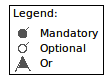
\includegraphics[width=.2\textwidth]{imagens/fm-hpl2.png}
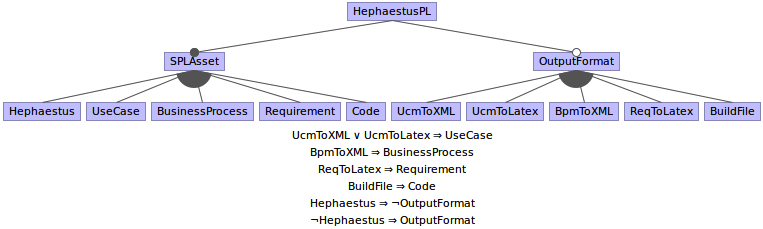
\includegraphics[width=\textwidth]{imagens/fm-hpl1.png}
\end{center}
\caption{\hpl's feature model. In this version, the features \textit{SPLAsset} and \textit{OutputFormat} define an \emph{or} relationship with their children}
\label{fig:hephaestus-fm-03}
\end{figure*}

%%%%%%%%%%%%%%%%%%%%%%%%%%%%%%%%%%%%%%%%%%%%%%%%%%

\subsection{\hpl's Feature Model} 
\label{feature-model-hpl}

In terms of the problem space, \hpl's feature model is represented in Figure~\ref{fig:hephaestus-fm-03}. As the diagram shows, the features \emph{SPLAsset} and \emph{OutputFormat} are mandatory. Further, these features are parents of \emph{or-features} so that combination of models and output formats are supported, e.g., a given instance might comprise business processes and use cases and export both assets as XML files. Managing variabilities in such a combination of features is essential in \hpl{} and has not been addressed elsewhere.

%%%%%%%%%%%%%%%%%%%%%%%%%%%%%%%%%%%%%%%%%%%%%%%%%%

\begin{figure*}[t!]
\begin{center}
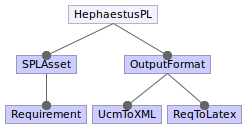
\includegraphics[scale=0.6]{imagens/confInvalid.png}
\end{center}
\caption{An invalid configuration of \hpl}
\label{fig:hephaestus-conf-invalid}
\end{figure*}

%%%%%%%%%%%%%%%%%%%%%%%%%%%%%%%%%%%%%%%%%%%%%%%%%%

In addition to the feature diagram, Figure~\ref{fig:hephaestus-fm-03} shows some cross-tree constraints that must be satisfied for any valid feature configuration of \hpl.  To illustrate, Figure~\ref{fig:hephaestus-conf1a} and Figure~\ref{fig:hephaestus-conf1b} show two valid configurations of \hpl, whereas Figure~\ref{fig:hephaestus-conf-invalid} shows an invalid configuration of \hpl, in which the \emph{UcmToXML} feature is selected, but the \emph{UseCase} feature is not selected. In this case, the $UcmToXML \lor UcmToLatex \rightarrow Use Case$ constraint was violated, leading to an invalid feature configuration of \hpl.

Thus, in the problem space, a specific configuration of \hp{} is conceptually simple in that it is represented by a combination of a few \textit{or-features}. However, in the solution space, a specific configuration implies more complexity because it require management of variability in several artifacts (algebraic data types, functions of different kinds, and models) at different levels of granularity (i.e., course-grained and fine-grained). As the change impact of the evolution scenario in Section~\ref{sec:hp-evolution} showed, the implementation of the features is somewhat scattered in \hp' source code.

%%%%%%%%%%%%%%%%%%%%%%%%%%%%%%%%%%%%%%%%%%%%%%%%%%

\subsection{Identification of Commonality} 
\label{sec:commonality}

In the solution space, there exists significant amount of commonality among configurations. 
The domain analysis revealed \emph{commonality} for these abstractions across the variants of the evolution history:

\begin{description}

\item[\emph{Feature Model Representation}] An algebraic data type represents the feature model of a product line.
  
\item[\emph{Product Configuration Representation}] An algebraic data type represents a valid feature configuration.

\item[\emph{CK Representation}] An algebraic data type represents the product line's configuration knowledge.

\item[\emph{Interpreter for Product Instantiation}] The \texttt{build} function performs the SPL instantiation by generating a product corresponding to a specific product line configuration.

\end{description}

%%%%%%%%%%%%%%%%%%%%%%%%%%%%%%%%%%%%%%%%%%%%%%%%%%

\subsection{Identification of Variability} 
\label{sec:variability}

The domain analysis revealed \emph{variability} for these abstractions across the variants of the evolution history:

\newcommand{\assetr}{\emph{Asset Representations}}
\newcommand{\assetx}{\emph{Asset Transformations}}
\newcommand{\asseti}{\emph{Asset Input}}
\newcommand{\asseto}{\emph{Asset Output}}
\newcommand{\assetc}{\emph{Asset Containers}}
\newcommand{\emptyi}{\emph{Empty Instance}}
\newcommand{\ckparser}{\emph{CK Parser}}

\begin{description}

\item[\assetr] Algebraic data types represent the abstract syntax of different SPL assets (such as use cases, business processes, and code).

\item[\assetx] Functions manipulate such artifacts, thereby resolving variability of SPL assets. Some transformations basically select a specific asset from the product line so that it is included into the product during derivation. Other transformations change the structure of an asset of the SPL in the final product.

\item[\assetc] The \texttt{SPLModel} and \texttt{InstanceModel} algebraic data types comprise the set of SPL assets and group it with the feature model or feature configuration, respectively, of a given \hpl{} instance.

\item[\asseti] Input functions for reading assets, possibly parsing the concrete syntax of an asset to the corresponding abstract syntax of \hpl{}, i.e., the asset abstract data types. Input functions are typically invoked upon starting product derivation so that all assets are made available to the process through a \texttt{SPLModel} value.

\item[\asseto] Output functions for writing artifacts in different output formats. Output functions are typically invoked upon finishing product derivation so that the derived product is persisted.

\item[\emptyi] An expression defines the initial representation of a product during the product derivation activity. It is an instance of the \texttt{InstanceModel} data type and serves as a baseline that is successively refined by the \texttt{build} function.

\item[\ckparser] The \texttt{xml2Transformation} function parses the XML representation of transformations into actual transformations (functions) on instance models for use in the configuration knowledge.

\end{description}

Domain analysis also substantiated that variability has a regular form that may be understood linguistically in terms of introduction of new abstractions (`modules') and extension of existing abstractions (data types and functions). For example, to introduce variability support for one new asset in \hp, one needs to implement the data types for representing the abstract syntax of these models, implement the transformations for solving variability, implement the parser and output functions for reading/writing these assets into/from \hp; one also needs to extend some data types and functions of \hp{}, as it was illustrated in Section~\ref{sec:hp-evolution}.
